\documentclass[11pt]{article}

\newcommand{\titrechapitre}{Géométrie dans le plan -- Cours}
\newcommand{\titreclasse}{Lycée Jean-Baptiste \textsc{Corot} -- Seconde $11$}
\newcommand{\pagination}{\thepage/\pageref{LastPage}}
\newcommand{\topbotmargins}{2cm}
\newcommand{\spacebelowexo}{5mm}
%%%%%%%%%%%%%%%%%%%%%%%%%%%%%%%%%%%%%%%%%%%%%%%%%%%%%%%%%%%%%%%%%%%%%%%%%%%%%%%%
%
% PACKAGES
% ========
%
%%%%%%%%%%%%%%%%%%%%%%%%%%%%%%%%%%%%%%%%%%%%%%%%%%%%%%%%%%%%%%%%%%%%%%%%%%%%%%%%

\usepackage[english, french]{babel}
\usepackage[utf8]{inputenc}
\usepackage[T1]{fontenc}
\usepackage{graphicx}
\usepackage{amsmath,amssymb,amsthm,amsopn}
\usepackage{hyperref}

% Pour avoir l'écriture \mathscr (math script)
% ============================================

\usepackage{mathrsfs}

% Deal with coma as a decimal separator
% =====================================

\usepackage{icomma}

% Package Geometry
% ================

\usepackage[a4paper, lmargin=2cm, rmargin=2cm, top=\topbotmargins, bottom=\topbotmargins]{geometry}

% Package multicol
% ================

\usepackage{multicol}

% Redefine abstract
% =================

% Note
% ====
%
% Le reste a été commenté pour ne pas charger trop de choses au démarrage. On
% verra si on en a besoin plus tard.
%
% --------
%
%\usepackage{mathrsfs}
%\usepackage{multirow}
%\usepackage{bm}
%\hypersetup{
%    colorlinks=true,
%    linkcolor=blue,
%    citecolor=red,
%}
%\usepackage{diagbox}
%
%\usepackage{algorithm}
%\usepackage{algpseudocode}
%
%\renewcommand{\algorithmicrequire}{\textbf{Input:}}
%\renewcommand{\algorithmicensure}{\textbf{Output:}}


%%%%%%%%%%%%%%%%%%%%%%%%%%%%%%%%%%%%%%%%%%%%%%%%%%%%%%%%%%%%%%%%%%%%%%%%%%%%%%%%
%
% TIKZ
% ====
%
%%%%%%%%%%%%%%%%%%%%%%%%%%%%%%%%%%%%%%%%%%%%%%%%%%%%%%%%%%%%%%%%%%%%%%%%%%%%%%%%

\usepackage{tikz}
\usetikzlibrary{arrows}

\usepackage{tkz-tab} % Variation tables

\usepackage{pgfplots}
%\usepackage{pgf-pie} % Pie charts

\pgfplotsset{
%\newcommand{\settingsgraph}{
x=.5cm,y=.5cm,
xticklabel style = {font=\scriptsize, yshift=.1cm},
yticklabel style = {font=\scriptsize, xshift=.1cm},
axis lines=middle,
ymajorgrids=true,
xmajorgrids=true,
major grid style = {color=white!80!blue},
xmin=-5.5,
xmax=5.5,
ymin=-5.5,
ymax=5.5,
xtick={-5.0,-4.0,...,5.0},
ytick={-5.0,-4.0,...,5.0},
}

% Tikz style

\tikzset{round/.style={circle, draw=black, very thick, scale = 0.7}}
\tikzset{arrow/.style={->, >=latex}}
\tikzset{dashed-arrow/.style={->, >=latex, dashed}}

\newcommand{\point}[3]{\draw[very thick, #3] (#1-.1, #2)--(#1+.1, #2)
(#1, #2-.1)--(#1, #2+.1)}

%%%%%%%%%%%%%%%%%%%%%%%%%%%%%%%%%%%%%%%%%%%%%%%%%%%%%%%%%%%%%%%%%%%%%%%%%%%%%%%%
%
% FANCY HEADER
% ============
%
%%%%%%%%%%%%%%%%%%%%%%%%%%%%%%%%%%%%%%%%%%%%%%%%%%%%%%%%%%%%%%%%%%%%%%%%%%%%%%%%


\usepackage{fancyhdr}
\usepackage{lastpage}

\pagestyle{fancy}
\newcommand{\changefont}{\fontsize{9}{9}\selectfont}
\renewcommand{\headrulewidth}{0mm}
\renewcommand{\footrulewidth}{0mm}

\fancyhead[C]{}
\fancyhead[L]{\titreclasse}
\fancyhead[R]{\titrechapitre}
\fancyfoot[C]{}
\fancyfoot[L]{}
\fancyfoot[R]{\pagination}
\addtolength{\skip\footins}{20pt} % distance between text and footnotes

%%%%%%%%%%%%%%%%%%%%%%%%%%%%%%%%%%%%%%%%%%%%%%%%%%%%%%%%%%%%%%%%%%%%%%%%%%%%%%%%
%
% THEOREM STYLE
% =============
%
%%%%%%%%%%%%%%%%%%%%%%%%%%%%%%%%%%%%%%%%%%%%%%%%%%%%%%%%%%%%%%%%%%%%%%%%%%%%%%%%

\usepackage[tikz]{bclogo}
\usepackage{mdframed}

\usepackage{tcolorbox}
\tcbuselibrary{listings, breakable, theorems, skins}

%\newtheoremstyle{break}%
%{}{}%
%{\itshape}{}%
%{\bfseries}{}%  % Note that final punctuation is omitted.
%{\newline}{}

\newtheoremstyle{scbf}%
{}{}%
{}{}%
%{\scshape}{}%  % Note that final punctuation is omitted.
{\bfseries\scshape}{}%  % Note that final punctuation is omitted.
{\newline}{}

%\theoremstyle{break}
%\theoremstyle{plain}
%\newtheorem{thm}{Theorem}[section]
%\newtheorem{lm}[thm]{Lemma}
%\newtheorem{prop}[thm]{Proposition}
%\newtheorem{cor}[thm]{Corollary}

%\theoremstyle{scbf}
%\newtheorem{exo}{$\star$ Exercice}

%\theoremstyle{definition}
%\newtheorem{defi}[thm]{Definition}
%\newtheorem{ex}[thm]{Example}

%\theoremstyle{remark}
%\newtheorem{rem}[thm]{Remark}

% Defining the Remark environment
% ===============================

\newenvironment{rmq}
  {
    \begin{bclogo}[logo=\bcinfo, noborder=true]{Remarque}
  }
  {
    \end{bclogo}
  }

% Defining the exercise environment
% =================================

\newcounter{exos}
\setcounter{exos}{1}

\newenvironment{exo}
  {
    \begin{bclogo}[logo=\bccrayon, noborder=true]{Exercice \theexos}
  }
  {
    \end{bclogo}
    \addtocounter{exos}{1}
  }


% Redefining the proof environment from amsthm
% ============================================

\tcolorboxenvironment{proof}{
  blanker, breakable, before skip=10pt,after skip=10pt,
  borderline west={1mm}{0pt}{red},
  left=5mm,
}

% Defining the definition environment
% ===================================

\colorlet{coldef}{black!50!green}

\newcounter{defis}
\setcounter{defis}{1}

\newenvironment{defi}[1]
  {
    \begin{defihid}{{#1}}{\thedefis}
  }
  {
    \end{defihid}
    \addtocounter{defis}{1}
  }

\newtcolorbox{defihid}[2]{%
  empty,title={ {\bfseries Définition {#2}} ({#1})},attach boxed title to top left,
boxed title style={empty,size=minimal,toprule=2pt,top=4pt,
overlay={\draw[coldef,line width=2pt]
([yshift=-1pt]frame.north west)--([yshift=-1pt]frame.north east);}},
coltitle=coldef,
before=\par\medskip\noindent,parbox=false,boxsep=0pt,left=0pt,right=3mm,top=4pt,
breakable,pad at break*=0mm,vfill before first,
overlay unbroken={\draw[coldef,line width=1pt]
([yshift=-1pt]title.north east)--([xshift=-0.5pt,yshift=-1pt]title.north-|frame.east)
--([xshift=-0.5pt]frame.south east)--(frame.south west); },
overlay first={\draw[coldef,line width=1pt]
([yshift=-1pt]title.north east)--([xshift=-0.5pt,yshift=-1pt]title.north-|frame.east)
--([xshift=-0.5pt]frame.south east); },
overlay middle={\draw[coldef,line width=1pt] ([xshift=-0.5pt]frame.north east)
--([xshift=-0.5pt]frame.south east); },
overlay last={\draw[coldef,line width=1pt] ([xshift=-0.5pt]frame.north east)
--([xshift=-0.5pt]frame.south east)--(frame.south west);},%
}

\newenvironment{notation}
  {
    \begin{notationhid}{\thedefis}
  }
  {
    \end{notationhid}
    \addtocounter{defis}{1}
  }

\newtcolorbox{notationhid}[1]{%
  empty,title={Notation {#1}},attach boxed title to top left,
boxed title style={empty,size=minimal,toprule=2pt,top=4pt,
overlay={\draw[coldef,line width=2pt]
([yshift=-1pt]frame.north west)--([yshift=-1pt]frame.north east);}},
coltitle=coldef,fonttitle=\bfseries,
before=\par\medskip\noindent,parbox=false,boxsep=0pt,left=0pt,right=3mm,top=4pt,
breakable,pad at break*=0mm,vfill before first,
overlay unbroken={\draw[coldef,line width=1pt]
([yshift=-1pt]title.north east)--([xshift=-0.5pt,yshift=-1pt]title.north-|frame.east)
--([xshift=-0.5pt]frame.south east)--(frame.south west); },
overlay first={\draw[coldef,line width=1pt]
([yshift=-1pt]title.north east)--([xshift=-0.5pt,yshift=-1pt]title.north-|frame.east)
--([xshift=-0.5pt]frame.south east); },
overlay middle={\draw[coldef,line width=1pt] ([xshift=-0.5pt]frame.north east)
--([xshift=-0.5pt]frame.south east); },
overlay last={\draw[coldef,line width=1pt] ([xshift=-0.5pt]frame.north east)
--([xshift=-0.5pt]frame.south east)--(frame.south west);},%
}


% Defining the proposition, theorem, etc. environment
% ===================================================

\colorlet{colprop}{red!75!black}

\newcounter{props}
\setcounter{props}{1}

\newenvironment{prop}
  {
    \begin{prophid}{\theprops}
  }
  {
    \end{prophid}
    \refstepcounter{props}
  }

\newtcolorbox{prophid}[1]{%
empty,title={Propriété {#1}},attach boxed title to top left,
boxed title style={empty,size=minimal,toprule=2pt,top=4pt,
overlay={\draw[colprop,line width=2pt]
([yshift=-1pt]frame.north west)--([yshift=-1pt]frame.north east);}},
coltitle=colprop,fonttitle=\bfseries,
before=\par\medskip\noindent,parbox=false,boxsep=0pt,left=0pt,right=3mm,top=4pt,
breakable,pad at break*=0mm,vfill before first,
overlay unbroken={\draw[colprop,line width=1pt]
([yshift=-1pt]title.north east)--([xshift=-0.5pt,yshift=-1pt]title.north-|frame.east)
--([xshift=-0.5pt]frame.south east)--(frame.south west); },
overlay first={\draw[colprop,line width=1pt]
([yshift=-1pt]title.north east)--([xshift=-0.5pt,yshift=-1pt]title.north-|frame.east)
--([xshift=-0.5pt]frame.south east); },
overlay middle={\draw[colprop,line width=1pt] ([xshift=-0.5pt]frame.north east)
--([xshift=-0.5pt]frame.south east); },
overlay last={\draw[colprop,line width=1pt] ([xshift=-0.5pt]frame.north east)
--([xshift=-0.5pt]frame.south east)--(frame.south west);},%
}

\newenvironment{propadm}
  {
    \begin{propadmhid}{\theprops}
  }
  {
    \end{propadmhid}
    \refstepcounter{props}
  }

  \newtcolorbox{propadmhid}[1]{%
    empty,title={{\bfseries Propriété {#1}} (admise)},attach boxed title to top left,
boxed title style={empty,size=minimal,toprule=2pt,top=4pt,
overlay={\draw[colprop,line width=2pt]
([yshift=-1pt]frame.north west)--([yshift=-1pt]frame.north east);}},
coltitle=colprop,%fonttitle=\bfseries,
before=\par\medskip\noindent,parbox=false,boxsep=0pt,left=0pt,right=3mm,top=4pt,
breakable,pad at break*=0mm,vfill before first,
overlay unbroken={\draw[colprop,line width=1pt]
([yshift=-1pt]title.north east)--([xshift=-0.5pt,yshift=-1pt]title.north-|frame.east)
--([xshift=-0.5pt]frame.south east)--(frame.south west); },
overlay first={\draw[colprop,line width=1pt]
([yshift=-1pt]title.north east)--([xshift=-0.5pt,yshift=-1pt]title.north-|frame.east)
--([xshift=-0.5pt]frame.south east); },
overlay middle={\draw[colprop,line width=1pt] ([xshift=-0.5pt]frame.north east)
--([xshift=-0.5pt]frame.south east); },
overlay last={\draw[colprop,line width=1pt] ([xshift=-0.5pt]frame.north east)
--([xshift=-0.5pt]frame.south east)--(frame.south west);},%
}

\newenvironment{propnom}[1]
  {
    \begin{propnomhid}{#1}{\theprops}
  }
  {
    \end{propnomhid}
    \refstepcounter{props}
  }

\newtcolorbox{propnomhid}[2]{%
empty,title={{\bfseries Propriété {#2}} ({#1})},attach boxed title to top left,
boxed title style={empty,size=minimal,toprule=2pt,top=4pt,
overlay={\draw[colprop,line width=2pt]
([yshift=-1pt]frame.north west)--([yshift=-1pt]frame.north east);}},
coltitle=colprop,
before=\par\medskip\noindent,parbox=false,boxsep=0pt,left=0pt,right=3mm,top=4pt,
breakable,pad at break*=0mm,vfill before first,
overlay unbroken={\draw[colprop,line width=1pt]
([yshift=-1pt]title.north east)--([xshift=-0.5pt,yshift=-1pt]title.north-|frame.east)
--([xshift=-0.5pt]frame.south east)--(frame.south west); },
overlay first={\draw[colprop,line width=1pt]
([yshift=-1pt]title.north east)--([xshift=-0.5pt,yshift=-1pt]title.north-|frame.east)
--([xshift=-0.5pt]frame.south east); },
overlay middle={\draw[colprop,line width=1pt] ([xshift=-0.5pt]frame.north east)
--([xshift=-0.5pt]frame.south east); },
overlay last={\draw[colprop,line width=1pt] ([xshift=-0.5pt]frame.north east)
--([xshift=-0.5pt]frame.south east)--(frame.south west);},%
}




\newenvironment{thm}
  {
    \begin{thmhid}{\theprops}
  }
  {
    \end{thmhid}
    \refstepcounter{props}
  }

\newtcolorbox{thmhid}[1]{%
empty,title={Théorème {#1}},attach boxed title to top left,
boxed title style={empty,size=minimal,toprule=2pt,top=4pt,
overlay={\draw[colprop,line width=2pt]
([yshift=-1pt]frame.north west)--([yshift=-1pt]frame.north east);}},
coltitle=colprop,fonttitle=\bfseries,
before=\par\medskip\noindent,parbox=false,boxsep=0pt,left=0pt,right=3mm,top=4pt,
breakable,pad at break*=0mm,vfill before first,
overlay unbroken={\draw[colprop,line width=1pt]
([yshift=-1pt]title.north east)--([xshift=-0.5pt,yshift=-1pt]title.north-|frame.east)
--([xshift=-0.5pt]frame.south east)--(frame.south west); },
overlay first={\draw[colprop,line width=1pt]
([yshift=-1pt]title.north east)--([xshift=-0.5pt,yshift=-1pt]title.north-|frame.east)
--([xshift=-0.5pt]frame.south east); },
overlay middle={\draw[colprop,line width=1pt] ([xshift=-0.5pt]frame.north east)
--([xshift=-0.5pt]frame.south east); },
overlay last={\draw[colprop,line width=1pt] ([xshift=-0.5pt]frame.north east)
--([xshift=-0.5pt]frame.south east)--(frame.south west);},%
}

\newenvironment{thmadm}
  {
    \begin{thmadmhid}{\theprops}
  }
  {
    \end{thmadmhid}
    \refstepcounter{props}
  }

  \newtcolorbox{thmadmhid}[1]{%
    empty,title={{\bfseries Théorème {#1}} (admis)},attach boxed title to top left,
boxed title style={empty,size=minimal,toprule=2pt,top=4pt,
overlay={\draw[colprop,line width=2pt]
([yshift=-1pt]frame.north west)--([yshift=-1pt]frame.north east);}},
coltitle=colprop,%fonttitle=\bfseries,
before=\par\medskip\noindent,parbox=false,boxsep=0pt,left=0pt,right=3mm,top=4pt,
breakable,pad at break*=0mm,vfill before first,
overlay unbroken={\draw[colprop,line width=1pt]
([yshift=-1pt]title.north east)--([xshift=-0.5pt,yshift=-1pt]title.north-|frame.east)
--([xshift=-0.5pt]frame.south east)--(frame.south west); },
overlay first={\draw[colprop,line width=1pt]
([yshift=-1pt]title.north east)--([xshift=-0.5pt,yshift=-1pt]title.north-|frame.east)
--([xshift=-0.5pt]frame.south east); },
overlay middle={\draw[colprop,line width=1pt] ([xshift=-0.5pt]frame.north east)
--([xshift=-0.5pt]frame.south east); },
overlay last={\draw[colprop,line width=1pt] ([xshift=-0.5pt]frame.north east)
--([xshift=-0.5pt]frame.south east)--(frame.south west);},%
}

\newenvironment{thmnom}[1]
  {
    \begin{thmnomhid}{#1}{\theprops}
  }
  {
    \end{thmnomhid}
    \refstepcounter{props}
  }

\newtcolorbox{thmnomhid}[2]{%
empty,title={{\bfseries Théorème {#2}} ({#1})},attach boxed title to top left,
boxed title style={empty,size=minimal,toprule=2pt,top=4pt,
overlay={\draw[colprop,line width=2pt]
([yshift=-1pt]frame.north west)--([yshift=-1pt]frame.north east);}},
coltitle=colprop,
before=\par\medskip\noindent,parbox=false,boxsep=0pt,left=0pt,right=3mm,top=4pt,
breakable,pad at break*=0mm,vfill before first,
overlay unbroken={\draw[colprop,line width=1pt]
([yshift=-1pt]title.north east)--([xshift=-0.5pt,yshift=-1pt]title.north-|frame.east)
--([xshift=-0.5pt]frame.south east)--(frame.south west); },
overlay first={\draw[colprop,line width=1pt]
([yshift=-1pt]title.north east)--([xshift=-0.5pt,yshift=-1pt]title.north-|frame.east)
--([xshift=-0.5pt]frame.south east); },
overlay middle={\draw[colprop,line width=1pt] ([xshift=-0.5pt]frame.north east)
--([xshift=-0.5pt]frame.south east); },
overlay last={\draw[colprop,line width=1pt] ([xshift=-0.5pt]frame.north east)
--([xshift=-0.5pt]frame.south east)--(frame.south west);},%
}

\newenvironment{coro}
  {
    \begin{corohid}{\theprops}
  }
  {
    \end{corohid}
    \refstepcounter{props}
  }

  \newtcolorbox{corohid}[1]{%
  empty,title={Corollaire {#1}},attach boxed title to top left,
boxed title style={empty,size=minimal,toprule=2pt,top=4pt,
overlay={\draw[colprop,line width=2pt]
([yshift=-1pt]frame.north west)--([yshift=-1pt]frame.north east);}},
coltitle=colprop,fonttitle=\bfseries,
before=\par\medskip\noindent,parbox=false,boxsep=0pt,left=0pt,right=3mm,top=4pt,
breakable,pad at break*=0mm,vfill before first,
overlay unbroken={\draw[colprop,line width=1pt]
([yshift=-1pt]title.north east)--([xshift=-0.5pt,yshift=-1pt]title.north-|frame.east)
--([xshift=-0.5pt]frame.south east)--(frame.south west); },
overlay first={\draw[colprop,line width=1pt]
([yshift=-1pt]title.north east)--([xshift=-0.5pt,yshift=-1pt]title.north-|frame.east)
--([xshift=-0.5pt]frame.south east); },
overlay middle={\draw[colprop,line width=1pt] ([xshift=-0.5pt]frame.north east)
--([xshift=-0.5pt]frame.south east); },
overlay last={\draw[colprop,line width=1pt] ([xshift=-0.5pt]frame.north east)
--([xshift=-0.5pt]frame.south east)--(frame.south west);},%
}

\newenvironment{lemme}
  {
    \begin{lemmehid}{\theprops}
  }
  {
    \end{lemmehid}
    \refstepcounter{props}
  }

  \newtcolorbox{lemmehid}[1]{%
  empty,title={Lemme {#1}},attach boxed title to top left,
boxed title style={empty,size=minimal,toprule=2pt,top=4pt,
overlay={\draw[colprop,line width=2pt]
([yshift=-1pt]frame.north west)--([yshift=-1pt]frame.north east);}},
coltitle=colprop,fonttitle=\bfseries,
before=\par\medskip\noindent,parbox=false,boxsep=0pt,left=0pt,right=3mm,top=4pt,
breakable,pad at break*=0mm,vfill before first,
overlay unbroken={\draw[colprop,line width=1pt]
([yshift=-1pt]title.north east)--([xshift=-0.5pt,yshift=-1pt]title.north-|frame.east)
--([xshift=-0.5pt]frame.south east)--(frame.south west); },
overlay first={\draw[colprop,line width=1pt]
([yshift=-1pt]title.north east)--([xshift=-0.5pt,yshift=-1pt]title.north-|frame.east)
--([xshift=-0.5pt]frame.south east); },
overlay middle={\draw[colprop,line width=1pt] ([xshift=-0.5pt]frame.north east)
--([xshift=-0.5pt]frame.south east); },
overlay last={\draw[colprop,line width=1pt] ([xshift=-0.5pt]frame.north east)
--([xshift=-0.5pt]frame.south east)--(frame.south west);},%
}

\colorlet{colexemple}{blue!50!black}
%\newtcolorbox{exemple}{empty, title=Exemple, attach boxed title to top left,
%  boxed title style={empty, size=minimal, toprule=2pt, top=4pt,
%    overlay={\draw[colexemple,line width=2pt]
%([yshift=-1pt]frame.north west)--([yshift=-1pt]frame.north east);}},
%coltitle=colexemple,fonttitle=\bfseries,%\large\bfseries,
%before=\par\medskip\noindent,parbox=false,boxsep=0pt,left=0pt,right=3mm,top=4pt,
%overlay={\draw[colexemple,line width=1pt]
%([yshift=-1pt]title.north east)--([xshift=-0.5pt,yshift=-1pt]title.north-|frame.east)
%--([xshift=-0.5pt]frame.south east)--(frame.south west); },
%}

\newcounter{exemples}
\setcounter{exemples}{1}

\newenvironment{exemple}
  {
    \begin{exemplehid}{\theexemples}
  }
  {
    \end{exemplehid}
    \addtocounter{exemples}{1}
  }

\newtcolorbox{exemplehid}[1]{%
empty,title={Exemple {#1}},attach boxed title to top left,
boxed title style={empty,size=minimal,toprule=2pt,top=4pt,
overlay={\draw[colexemple,line width=2pt]
([yshift=-1pt]frame.north west)--([yshift=-1pt]frame.north east);}},
coltitle=colexemple,fonttitle=\bfseries,
before=\par\medskip\noindent,parbox=false,boxsep=0pt,left=0pt,right=3mm,top=4pt,
breakable,pad at break*=0mm,vfill before first,
overlay unbroken={\draw[colexemple,line width=1pt]
([yshift=-1pt]title.north east)--([xshift=-0.5pt,yshift=-1pt]title.north-|frame.east)
--([xshift=-0.5pt]frame.south east)--(frame.south west); },
overlay first={\draw[colexemple,line width=1pt]
([yshift=-1pt]title.north east)--([xshift=-0.5pt,yshift=-1pt]title.north-|frame.east)
--([xshift=-0.5pt]frame.south east); },
overlay middle={\draw[colexemple,line width=1pt] ([xshift=-0.5pt]frame.north east)
--([xshift=-0.5pt]frame.south east); },
overlay last={\draw[colexemple,line width=1pt] ([xshift=-0.5pt]frame.north east)
--([xshift=-0.5pt]frame.south east)--(frame.south west);},%
}

\newenvironment{contrex}
  {
    \begin{contrexhid}{\theexemples}
  }
  {
    \end{contrexhid}
    \addtocounter{exemples}{1}
  }

\newtcolorbox{contrexhid}[1]{%
empty,title={Contre-exemple {#1}},attach boxed title to top left,
boxed title style={empty,size=minimal,toprule=2pt,top=4pt,
overlay={\draw[colexemple,line width=2pt]
([yshift=-1pt]frame.north west)--([yshift=-1pt]frame.north east);}},
coltitle=colexemple,fonttitle=\bfseries,
before=\par\medskip\noindent,parbox=false,boxsep=0pt,left=0pt,right=3mm,top=4pt,
breakable,pad at break*=0mm,vfill before first,
overlay unbroken={\draw[colexemple,line width=1pt]
([yshift=-1pt]title.north east)--([xshift=-0.5pt,yshift=-1pt]title.north-|frame.east)
--([xshift=-0.5pt]frame.south east)--(frame.south west); },
overlay first={\draw[colexemple,line width=1pt]
([yshift=-1pt]title.north east)--([xshift=-0.5pt,yshift=-1pt]title.north-|frame.east)
--([xshift=-0.5pt]frame.south east); },
overlay middle={\draw[colexemple,line width=1pt] ([xshift=-0.5pt]frame.north east)
--([xshift=-0.5pt]frame.south east); },
overlay last={\draw[colexemple,line width=1pt] ([xshift=-0.5pt]frame.north east)
--([xshift=-0.5pt]frame.south east)--(frame.south west);},%
}

\newenvironment{app}
  {
    \begin{apphid}{\theexemples}
  }
  {
    \end{apphid}
    \addtocounter{exemples}{1}
  }

\newtcolorbox{apphid}[1]{%
empty,title={Application {#1}},attach boxed title to top left,
boxed title style={empty,size=minimal,toprule=2pt,top=4pt,
overlay={\draw[colexemple,line width=2pt]
([yshift=-1pt]frame.north west)--([yshift=-1pt]frame.north east);}},
coltitle=colexemple,fonttitle=\bfseries,
before=\par\medskip\noindent,parbox=false,boxsep=0pt,left=0pt,right=3mm,top=4pt,
breakable,pad at break*=0mm,vfill before first,
overlay unbroken={\draw[colexemple,line width=1pt]
([yshift=-1pt]title.north east)--([xshift=-0.5pt,yshift=-1pt]title.north-|frame.east)
--([xshift=-0.5pt]frame.south east)--(frame.south west); },
overlay first={\draw[colexemple,line width=1pt]
([yshift=-1pt]title.north east)--([xshift=-0.5pt,yshift=-1pt]title.north-|frame.east)
--([xshift=-0.5pt]frame.south east); },
overlay middle={\draw[colexemple,line width=1pt] ([xshift=-0.5pt]frame.north east)
--([xshift=-0.5pt]frame.south east); },
overlay last={\draw[colexemple,line width=1pt] ([xshift=-0.5pt]frame.north east)
--([xshift=-0.5pt]frame.south east)--(frame.south west);},%
}

%%%%%%%%%%%%%%%%%%%%%%%%%%%%%%%%%%%%%%%%%%%%%%%%%%%%%%%%%%%%%%%%%%%%%%%%%%%%%%%%
%
% ENUMERATE
% =========
%
%%%%%%%%%%%%%%%%%%%%%%%%%%%%%%%%%%%%%%%%%%%%%%%%%%%%%%%%%%%%%%%%%%%%%%%%%%%%%%%%

\usepackage{enumerate}
\usepackage{enumitem}

% To have special enumerate items like
%
% 1/
% 2/
% 3/

%%%%%%%%%%%%%%%%%%%%%%%%%%%%%%%%%%%%%%%%%%%%%%%%%%%%%%%%%%%%%%%%%%%%%%%%%%%%%%%%
%
% ARRAYS
% ======
%
%%%%%%%%%%%%%%%%%%%%%%%%%%%%%%%%%%%%%%%%%%%%%%%%%%%%%%%%%%%%%%%%%%%%%%%%%%%%%%%%


\usepackage{array}
\usepackage{makecell} % Used to break lines within arrays
\usepackage{multirow}
\usepackage{booktabs} % Used to have nice arrays with headrules

%%%%%%%%%%%%%%%%%%%%%%%%%%%%%%%%%%%%%%%%%%%%%%%%%%%%%%%%%%%%%%%%%%%%%%%%%%%%%%%%
%
% WRITE CODE
% ==========
%
%%%%%%%%%%%%%%%%%%%%%%%%%%%%%%%%%%%%%%%%%%%%%%%%%%%%%%%%%%%%%%%%%%%%%%%%%%%%%%%%

\usepackage{listings}
\usepackage{xcolor}

%New colors defined below
\definecolor{codegreen}{rgb}{0,0.6,0}
\definecolor{codegray}{rgb}{0.5,0.5,0.5}
\definecolor{codepurple}{rgb}{0.58,0,0.82}
\definecolor{backcolour}{rgb}{0.95,0.95,0.92}

%Code listing style named "mystyle"
\lstdefinestyle{python}{
  %backgroundcolor=\color{backcolour},
  commentstyle=\color{codegreen},
  keywordstyle=\color{magenta},
  numberstyle=\tiny\color{codegray},
  stringstyle=\color{codepurple},
  basicstyle=\ttfamily\footnotesize,
  breakatwhitespace=false,
  breaklines=true,
  captionpos=b,
  keepspaces=true,
  numbers=left,
  numbersep=5pt,
  showspaces=false,
  showstringspaces=false,
  showtabs=false,
  tabsize=2
}

\lstset{style=python}

%%%%%%%%%%%%%%%%%%%%%%%%%%%%%%%%%%%%%%%%%%%%%%%%%%%%%%%%%%%%%%%%%%%%%%%%%%%%%%%%
%
% Tabular 
% =======
%
%%%%%%%%%%%%%%%%%%%%%%%%%%%%%%%%%%%%%%%%%%%%%%%%%%%%%%%%%%%%%%%%%%%%%%%%%%%%%%%%

% In order to obtain a tabular with given width.

\usepackage{tabularx}
\newcolumntype{Y}{>{\centering\arraybackslash}X}
\newcolumntype{R}{>{\raggedright\arraybackslash}X}
\newcolumntype{L}{>{\raggedleft\arraybackslash}X}
% \usepackage{tabulary} % younger brother

%%%%%%%%%%%%%%%%%%%%%%%%%%%%%%%%%%%%%%%%%%%%%%%%%%%%%%%%%%%%%%%%%%%%%%%%%%%%%%%%
%
% MACROS
% ======
%
%%%%%%%%%%%%%%%%%%%%%%%%%%%%%%%%%%%%%%%%%%%%%%%%%%%%%%%%%%%%%%%%%%%%%%%%%%%%%%%%

% Math Operators

\DeclareMathOperator{\Card}{Card}
\DeclareMathOperator{\Gal}{Gal}
\DeclareMathOperator{\Id}{Id}
\DeclareMathOperator{\Img}{Im}
\DeclareMathOperator{\Ker}{Ker}
\DeclareMathOperator{\Minpoly}{Minpoly}
\DeclareMathOperator{\Mod}{mod}
\DeclareMathOperator{\Ord}{Ord}
\DeclareMathOperator{\ppcm}{ppcm}
\DeclareMathOperator{\pgcd}{pgcd}
\DeclareMathOperator{\tr}{Tr}
\DeclareMathOperator{\Vect}{Vect}
\DeclareMathOperator{\Span}{Span}
\DeclareMathOperator{\rank}{rank}
\DeclareMathOperator{\rg}{rg}
\DeclareMathOperator{\ev}{ev}
\DeclareMathOperator{\Var}{Var}

% Shortcuts

\newcommand{\eg}{\emph{e.g. }}
\newcommand{\ent}[2]{[\![#1,#2]\!]}
\newcommand{\ie}{\emph{i.e. }}
\newcommand{\ps}[2]{\left\langle#1,#2\right\rangle}
\newcommand{\eqdef}{\overset{\text{def}}{=}}
\newcommand{\E}{\mathcal{E}}
\newcommand{\M}{\mathcal{M}}
\newcommand{\A}{\mathcal{A}}
\newcommand{\B}{\mathcal{B}}
\newcommand{\R}{\mathcal{R}}
\newcommand{\D}{\mathcal{D}}
\newcommand{\Pcal}{\mathcal{P}}
\newcommand{\K}{\mathbf{k}}
\newcommand{\vect}[1]{\overrightarrow{#1}}



\title{\vspace{-15mm}Chapitre 3 : Géométrie dans le plan}
\date{\vspace{-14mm}
\href{https://erou.forge.aeif.fr/s11/geom.html}{
  
\includegraphics[scale=.6]{qr-géométrie-plan.png}}
\vspace{-12mm}}
\author{}

%TODO: ajouter une application avec une question du type calculer les
% coordonnées du point C tel que B soit le milieu de [AC] (A et B étant connus).
% C'est-à-dire une résolution d'équation.
%
% Autre : pendant la trigonométrie, utiliser des exemples où on a pas le
% choix de la fonction trigonométrique à utiliser. Le mettre dans les exos
% aussi j'imagine.
%
% Encore : mettre un exemple d'utilisation de la propriété
% cos^2(a)+sin^2(a) = 1.

\begin{document}
\maketitle\thispagestyle{fancy}

\section{Coordonnées d'un point du plan}
\subsection{Repères du plan}

\begin{defi}{Repère, origine, et axes}
  Soient $O$, $I$ et $J$ trois points distincts du plan. On dit que le triplet
  $(O; I, J)$ forme un repère du plan lorsque les points $O$, $I$, et $J$ ne
  sont pas alignés. Dans ce cas :
  \begin{itemize}
    \item le point $O$ est \textbf{l'origine} du repère ;
    \item la droite orientée $(OI)$ est \textbf{l'axe des abscisses} et la
      distance $OI$ donne l'unité sur cet axe ;
    \item la droite orientée $(OJ)$ est \textbf{l'axe des ordonnées} et la
      distance OJ donne l'unité sur cet axe.
  \end{itemize}
\end{defi}

\begin{defi}{Coordonnées}
  \label{defi1}
  \begin{minipage}{.5\textwidth}
  Repérer un point $M$ dans un repère $(O; I, J)$, c'est donner l'unique couple
  de nombres réels $(x; y)$ appelé \textbf{coordonnées} du point $M$. Le nombre
  $x$ est \textbf{l'abscisse} du point $M$ et le nombre $y$ est
  \textbf{l'ordonnée} du point $M$.
  \end{minipage}
  \begin{minipage}{.5\textwidth}
    \begin{center}
      \begin{tikzpicture}[scale=.5]
      \draw[thick] (0,-2.4) -- (0, 4.4);
      \draw[thick] (-2.4,0) -- (6.6, 0);
      \foreach \x in {-1, ..., 3}{
      \draw[blue, opacity=.3] (2*\x, -2.4) -- (2*\x, 4.4);
      \draw[thick] (2*\x, -.2) -- (2*\x, .2);
      }
      \foreach \x in {-1, ..., 2}{
      \draw[blue, opacity=.3] (-2.4, 2*\x) -- (6.6, 2*\x);
      \draw[black, thick] (-.2, 2*\x) -- (.2, 2*\x);
      }
      \node (O) at (-.5,-.5) {$O$};
      \node (I) at (2,-.5) {$I$};
      \node (J) at (-.5,2) {$J$};

      \draw[thick] (3.8, -2) -- (4.2, -2) (4, -2.2) -- (4, -1.8);
      \draw[thick, loosely dashed] (0, -2) -- (4, -2) -- (4, 0);

      \node (M) at (4.4, -1.6) {$M$};
      \node (x) at (4, .5) {$x$};
      \node (y) at (-.5, -2) {$y$};
    \end{tikzpicture}
    \end{center}
  \end{minipage}
\end{defi}

\begin{app}
  Dans le repère juste au-dessus, donner les coordonnées des points $O$, $I$, $J$, et
  $M$.
\end{app}

\begin{rmq}
  Si les droites $(OI)$ et $(OJ)$ sont perpendiculaires, le repère $(O; I, J)$
  est \textbf{orthogonal}. Si, de plus, les longueurs $OI$ et $OJ$ sont égales,
  alors $(O; I, J)$ est dit \textbf{orthonormé}.
\end{rmq}

\begin{notation}
  On écrit souvent les coordonnées d'un point $A$ à l'aide de la notation
  $A(x_A; y_A)$.
\end{notation}

\begin{app}~\\[-6mm]
  \begin{minipage}{.5\textwidth}
    \begin{itemize}
      \item L'ordonnée du point $A$ est :
      \item L'abscisse du point $B$ est :
      \item Les coordonnées de $C$ sont :
      \item Les coordonnees de $D$ sont :
    \end{itemize}
\end{minipage}
  \begin{minipage}{.5\textwidth}
    \begin{center}
      \begin{tikzpicture}[scale=.5]
      \draw[semithick] (0,-4.4) -- (0, 4.4);
      \draw[semithick] (-4.4,0) -- (4.4, 0);
      \foreach \x in {-2, ..., 2}{
      \draw[blue, thin, opacity=.3] (2*\x, -4.4) -- (2*\x, 4.4);
      \draw[semithick] (2*\x, -.2) -- (2*\x, .2);
      }
      \foreach \x in {-2, ..., 2}{
      \draw[blue, thin, opacity=.3] (-4.4, 2*\x) -- (4.4, 2*\x);
      \draw[black, semithick] (-.2, 2*\x) -- (.2, 2*\x);
      }
      \node (O) at (-.5,-.5) {$O$};
      \node (I) at (2,-.5) {$I$};
      \node (J) at (-.5,2) {$J$};

      \draw[ultra thick, red] (1.8, 4) -- (2.2, 4) (2, 4.2) -- (2, 3.8);
      \node[red] (A) at (2.4, 3.5) {$A$};
      \draw[ultra thick, red] (-.2, -4) -- (.2, -4) (0, -4.2) -- (0, -3.8);
      \node[red] (B) at (.4, -3.5) {$B$};
      \draw[ultra thick, red] (-4.2, 0) -- (-3.8, 0) (-4, -.2) -- (-4, .2);
      \node[red] (C) at (-3.6, .5) {$C$};
      \draw[ultra thick, red] (-2.2, 4) -- (-1.8, 4) (-2, 4.2) -- (-2, 3.8);
      \node[red] (D) at (-1.6, 3.5) {$D$};
    \end{tikzpicture}
    \end{center}
  \end{minipage}
\end{app}

\subsection{Coordonnées du milieu d'un segment}
\begin{prop}
  Dans le plan muni d'un repère $(O; I, J)$, on considère les points $A(x_A;
  y_A)$ et $B(x_B; y_B)$. Le milieu $K$ du segment $\left[ AB \right]$ a pour
  coordonnées $(x_K; y_K)$ définies par
  \[
    x_K = \frac{x_A+x_B}{2}\text{ et }y_K = \frac{y_A+y_B}{2}.
  \]
\end{prop}
\begin{rmq}
  L'abscisse de $K$ est la moyenne des abscisses de $A$ et $B$. L'ordonnée de
  $K$ est la moyenne des ordonnées de $A$ et $B$.
\end{rmq}
\begin{app}~\\[-5mm]
  \begin{minipage}{.6\textwidth}
  Soient $A(1; 1)$, $B(-2; 0)$, $C(-1; -2)$ et $D(2; -1)$ quatre points dans un
  repère $(O; I, J)$.
  \begin{enumerate}
    \item Placer ces points dans le repère ci-contre.
    \item Calculer les coordonnées de $K$, le milieu de $\left[ AC \right]$.
    \item Calculer les coordonnées de $L$, le milieu de $\left[ BD \right]$.
    \item Le quadrilatère $ABCD$ est-il un parallélogramme ?
  \end{enumerate}
\end{minipage}
  \begin{minipage}{.4\textwidth}
    \begin{center}
      \begin{tikzpicture}[scale=.5]
      \draw[semithick] (0,-4.4) -- (0, 4.4);
      \draw[semithick] (-4.4,0) -- (4.4, 0);
      \foreach \x in {-2, ..., 2}{
      \draw[blue, thin, opacity=.3] (2*\x, -4.4) -- (2*\x, 4.4);
      \draw[semithick] (2*\x, -.2) -- (2*\x, .2);
      }
      \foreach \x in {-2, ..., 2}{
      \draw[blue, thin, opacity=.3] (-4.4, 2*\x) -- (4.4, 2*\x);
      \draw[black, semithick] (-.2, 2*\x) -- (.2, 2*\x);
      }
      \node (O) at (-.5,-.5) {$O$};
      \node (I) at (2,-.5) {$I$};
      \node (J) at (-.5,2) {$J$};
    \end{tikzpicture}
    \end{center}
  \end{minipage}
\end{app}

\section{Distance dans un repère orthonormé}
\begin{prop}
  %TODO: dessin pour voir ce que ça veut dire
  Dans un repère orthonormé du plan, la distance entre deux points $A$ et $B$ de
  coordonnées respectives $(x_A; y_A)$ et $(x_B; y_B)$ est donnée par
  \[
    AB = \sqrt{(x_B-x_A)^2+(y_B-y_A)^2}.
  \]
\end{prop}

\begin{app}
  Soit $(O; I, J)$ un repère orthonormé et $A(-1; 2)$ et $B(4; 3)$. Calculer la
  distance $AB$.
\end{app}

\begin{app}
  Dans un repère orthonormé $(O; I, J)$ du plan, on considère les points $A$,
  $B$, $C$ et $M$ de coordonnées respectives $(-2; 3)$, $(3; 4)$, $(3; -2)$ et
  $(1; 1)$.\\
  Montrer que $A$, $B$, et $C$ appartiennent à un même cercle de centre $M$.
\end{app}

\begin{prop}
  Soient $A$, $B$ et $C$ trois points distincts du plan. Les points $A$, $B$ et
  $C$ sont alignés dans cet ordre si, et seulement si, $AC = AB+BC$.
\end{prop}

\begin{app}
  Soit $(O; I, J)$ un repère orthonormé et $A(-2; -2)$, $B(3; 1)$ et
  $C(8; 4)$ trois points de ce repère.\\
  Ces points sont-ils alignés ?
\end{app}

\begin{app}~\\[-5mm]
  \begin{minipage}[]{.5\textwidth}
    Dans le repère orthonormé $(A; I, J)$, on considère la figure ci-contre
    composée d'un carrée $ABCD$ et de deux points $E$ et $F$. Les points $E$,
    $C$ et $F$ sont-ils alignés ?
  \end{minipage}
  \begin{minipage}[]{.5\textwidth}
    \begin{center}
       \begin{tikzpicture}[scale=.5]
      \draw[semithick] (0,-.25) -- (0, 7.25);
      \draw[semithick] (-.25,0) -- (10.75, 0);
      \foreach \x in {1, ..., 21}{
      \draw[blue, thin, opacity=.3] (.5*\x, -.25) -- (.5*\x, 7.25);
      \draw[semithick] (.5*\x, -.1) -- (.5*\x, .1);
      }
      \foreach \x in {5, 10,..., 20}{
      \node (\x) at (.5*\x, -.4) {$\x$};
      }
      \foreach \x in {0, 1, ..., 14}{
      \draw[blue, thin, opacity=.3] (-.25, .5*\x) -- (10.75, .5*\x);
      \draw[black, semithick] (-.1, .5*\x) -- (.1, .5*\x);
      }
      \foreach \x in {5, 10}{
      \node (\x) at (-.4, .5*\x) {$\x$};
      }
      \node (O) at (-.5,-.5) {$A$};
      \node (I) at (.5,-.5) {$I$};
      \node (J) at (-.5,.5) {$J$};

      \node (B) at (4,-.5) {$B$};
      \node (D) at (-.5,4) {$D$};

      \draw[semithick] (0, 6.5) -- (4, 4) -- (10.5, 0);

      \draw[thick] (3.9, 4) -- (4.1, 4) (4, 4.1) -- (4, 3.9);
      \node (C) at (4.3, 4.3) {$C$};
      \node (E) at (.4, 6.8) {$E$};
      \node (F) at (10.8, .3) {$F$};

      \fill[draw=orange, yellow!50!white, opacity=.4] (0,0) rectangle (4, 4);
    \end{tikzpicture}
    \end{center}
  \end{minipage}
\end{app}

\section{Configurations du plan}
\subsection{Propriétés dans le triangle}
\begin{defi}{Cercle circonscrit}
  Le \textbf{cercle circonscrit} à un triangle est le cercle passant par les
  trois sommets du triangle.
\end{defi}

\begin{prop}~\\[-7mm]
  \begin{minipage}{.5\textwidth}
  Dans un triangle, les médiatrices des côtés sont concourantes en un point $O$
  qui est le centre du \href{https://www.geogebra.org/m/wv4ccwvu}{cercle
  circonscrit} au triangle.
  \end{minipage}
  \begin{minipage}{.5\textwidth}
\begin{center}
  \begin{tikzpicture}
    \fill[green!50!black, opacity=.2] (-1,-1) -- (2, 1) -- (-2, 2);
    \draw[green!50!black, opacity=.8] (-1,-1) -- (2, 1) -- (-2, 2) -- (-1, -1);
    \draw[red!70!black] (-.14, .95) circle (2.138);

    \draw[red!30!black, opacity=.5] (1.33, -1.25) -- (-1.69, 3.29);
    \draw[red!30!black, opacity=.5] (.53, 3.62) -- (-.74, -1.45);
    \draw[red!30!black, opacity=.5] (-2.48, .17) -- (2.36, 1.79);

    \node[green!50!black] (A) at (-1.2, -1.2) {$A$};
    \node[green!50!black] (B) at (2.2, 1.2) {$B$};
    \node[green!50!black] (C) at (-2.2, 2.2) {$C$};

    \node[red!70!black] (O) at (.16, .85) {$O$};
  \end{tikzpicture}
\end{center}
  \end{minipage}
\end{prop}

\begin{defi}{Projeté orthogonal}
  \begin{minipage}{.5\textwidth}
  Soient $d$ une droite et $M$ un point extérieur à $d$. On dit que $M'$ est le
  \href{https://www.geogebra.org/m/cdcutrsn}{\textbf{projeté
  orthogonal}} de $M$ lorsque le point $M'$ appartient à la droit
  $d$ et que les droites $(MM')$ et $d$ sont perpendiculaires.
  \end{minipage}
  \begin{minipage}{.5\textwidth}
    \begin{center}
      \begin{tikzpicture}
        \draw[red!70!black] (-.71, -.66) -- (1.65, 1.55);
        \draw[blue!70!black, semithick] (-.53, 1.48) -- (-.33, 1.48) (-.43, 1.38) -- (-.43,
        1.58);
        \draw[dashed] (-.43, 1.48) -- (.5, .48);
        \draw[blue!70!black, semithick] (.4, .48) -- (.6, .48) (.5, .38) -- (.5,.58);

        \node[red!70!black] (d) at (1.6, 1.3) {$d$};
        \node[blue!70!black] (M) at (-.8, 1.2) {$M$};
        \node[blue!70!black] (M') at (1, .5) {$M'$};
      \end{tikzpicture}
    \end{center}
  \end{minipage}
\end{defi}

\begin{prop}
  Le projeté orthogonal d'un point $M$ sur une droite $d$ est le point de $d$ le
  plus proche de $M$.
\end{prop}

\begin{defi}{Hauteur}~\\[-4mm]
  \begin{minipage}{.5\textwidth}
    Dans un triangle $ABC$, la \textbf{hauteur} issue du sommet $A$ est la
    droite passant par $A$ et par $H$, le projeté orthogonal de $A$ sur $(BC)$ : il
    s'agit de la droite $(AH)$.
\end{minipage}
  \begin{minipage}{.5\textwidth}
\begin{center}
  \begin{tikzpicture}
    \fill[green!50!black, opacity=.2] (0,1) -- (-1.5, .5) -- (1, -1);
    \draw[green!50!black, opacity=.8] (0,1) -- (-1.5, .5) -- (1, -1) -- (0,1);
    \draw (-.78, -.3) -- (.26, 1.43);
    \node[green!50!black] (A) at (.3, 1.1) {\small $A$};
    \node[green!50!black] (B) at (-1.7, .6) {\small $B$};
    \node[green!50!black] (C) at (1.3, -.9) {\small $C$};
    \node (H) at (-.5, -.4) {\small $H$};
    \draw (-.55, .08) -- (-.43, .01) -- (-.5, -.1);
  \end{tikzpicture}
\end{center}
  \end{minipage}
\end{defi}

\newpage
\begin{app}~\\[-5mm]
  \begin{minipage}{.7\textwidth}
    On considère les points dans le repère ci-contre.
    \begin{enumerate}
      \item En utilisant les carreaux, justifier que la droite $(AT)$ est la
        médiatrice du segment $\left[ BC \right]$.
      \item Que peut-on déduire pour les droites $(BC)$ et $(AT)$ ?
    \end{enumerate}
  \end{minipage}
  \begin{minipage}{.3\textwidth}
    \begin{center}
      \begin{tikzpicture}[scale=.5]
      \foreach \x in {-3, ..., 3}{
      \draw[blue, thin, opacity=.3] (\x, -3.4) -- (\x, 3.4);
      }
      \foreach \x in {-3, ..., 3}{
      \draw[blue, thin, opacity=.3] (-3.4, \x) -- (3.4, \x);
      }

      \draw[thick] (-2.2, 0) -- (-1.8, 0) (-2, -.2) -- (-2, .2);
      \draw[thick] (-1.2, -3) -- (-0.8, -3) (-1, -3.2) -- (-1, -2.8);
      \draw[thick] (1.8, -2) -- (2.2, -2) (2, -2.2) -- (2, -1.8);
      \draw[thick] (1.8, 3) -- (2.2, 3) (2, 2.8) -- (2, 3.2);
      \node (A) at (2.5, 2.7) {\small $A$};
      \node (A) at (2.5, -1.4) {\small $B$};
      \node (A) at (-1.5, .4) {\small $C$};
      \node (A) at (-.5, -2.6) {\small $T$};
    \end{tikzpicture}
    \end{center}
  \end{minipage}

\end{app}

\subsection{Trigonométrie}
\begin{defi}{Cosinus et sinus}
  \begin{minipage}{.7\textwidth}
  Soit $ABC$ un triangle rectangle en $A$. On définit alors le \textbf{cosinus}
  et le \textbf{sinus} de l'angle $\widehat{ABC}$ de la façon suivante.
  \[
    \cos(\widehat{ABC})=\frac{AB}{BC}\text{ et }\sin(\widehat{ABC}) =
    \frac{AC}{BC}.
  \]
\end{minipage}
  \begin{minipage}{.3\textwidth}
\begin{center}
  \begin{tikzpicture}[scale=1.5]
    \fill[green!50!black, opacity=.2] (0,0) -- (0.95, .48) -- (-.5, 1);
    \draw[green!50!black, opacity=.8] (0,0) -- (0.95, .48) -- (-.5, 1) -- (0,0);
    \node[green!50!black] (A) at (-.4, 0) {\small $A$};
    \node[green!50!black] (B) at (1.3, .5) {\small $B$};
    \node[green!50!black] (C) at (-.7, 1) {\small $C$};
    \draw (-.08, .15) -- (0.08, .23) -- (.15, .08);
  \end{tikzpicture}
\end{center}
  \end{minipage}
\end{defi}

\begin{prop}
  Si $\alpha$ est la mesure d'un angle aigu dans un triangle rectangle alors
  $\cos^2(\alpha)+\sin^2(\alpha)=1$.
\end{prop}

\begin{app}
  \begin{enumerate}
    \item Démontrer que le triangle $ABC$ tel que $AB=12$, $BS=5$ et $AC=13$ est
      rectangle.
    \item Calculer la mesure de l'angle $\widehat{BAC}$.
  \end{enumerate}
\end{app}

\subsection{Quadrilatères}
\noindent\begin{minipage}{.5\textwidth}
  \begin{defi}{Parallélogramme}
    Un parallélogramme $ABCD$ est un quadrilatère dont les côtés opposés sont
    parallèles deux à deux.
  \end{defi}
  \begin{prop}
    Les diagonales d'un parallélogramme se coupent en leur milieu. Ce point est
    un centre de symétrie du quadrilatère. Ses côtés opposés sont de même
    longueur deux à deux.
  \end{prop}
  \begin{defi}{Autres parallélogrammes}
    Les carrés, les losanges et les rectangles sont des parallélogrammes. Toutes
    les propriétés des parallélogrammes s'appliquent à eux, mais ils vérifient
    aussi d'autres propriétés :\\
    \textbf{Rectangle :} tous ses angles sont droits et ses diagonales sont de
    même longueur.\\
    \textbf{Losange :} les diagonales sont perpendiculaires et tous ses côtés
    sont de même longueur.\\
    \textbf{Carré :} c'est à la fois un rectangle et un losange.
  \end{defi}
\end{minipage}
\begin{minipage}{.5\textwidth}
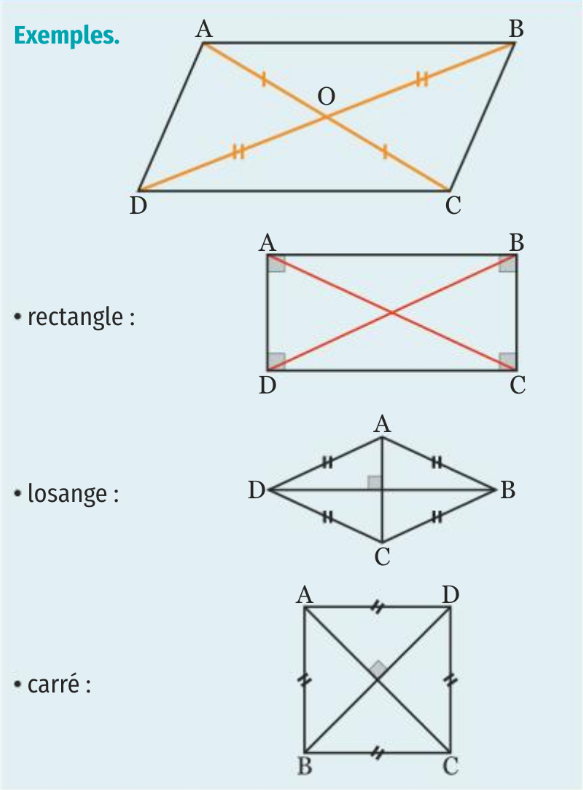
\includegraphics[scale=.4]{quadri.png}
\end{minipage}
\end{document}
